        % ------------------------------------------ %
        %                      (2.18)                %
        % ------------------------------------------ %
        Consider the sets of points $\left(x_1, x_2\right)$ whose `distances' from the origin are given by
        \[
            c^2 = 4x_1^2 + 3x_2^2 - 2\sqrt{2}x_1x_2
        \]
        for $c^2 = 1$ and for $c^2 = 4$. Determine the major and minor axes of the ellipses of constant
        distances and their associated lengths. Sketch the ellipses of constant distances and
        comment on their positions. What will happen as $c^2$ increases?
        \newline
        \par
        Converting the quadratic polynomial to a matrix,
        \[
            c^2 = 4x_1^2 + 3x_2^2 - 2\sqrt{2}x_1x_2
            =
            \begin{bmatrix}
                x_1 & x_2
            \end{bmatrix}
            \begin{bmatrix}
                4 & -\sqrt{2} \\
                -\sqrt{2} & 3
            \end{bmatrix}
            \begin{bmatrix}
                x_1 \\
                x_2
            \end{bmatrix}
            =
            \bold{x}^\prime\bold{A}\bold{x}
        \]
        Finding the eigenvalues and eigenvectors,
        \[
            0 = \left|\bold{A} - \lambda\bold{I}\right|
            =
            \left|
            \begin{matrix}
                4-\lambda & -\sqrt{2} \\
                -\sqrt{2} & 3-\lambda
            \end{matrix}
            \right|
            =
            \left(4-\lambda\right)\left(3-\lambda\right) - 2
            =
            \lambda^2 -7\lambda + 12 - 2 
            =
        \]
        \[
            =
            \left(\lambda-2\right)\left(\lambda-5\right)
        \]
        The eigenvalues are $\left\{\lambda_1, \lambda_2\right\} = \left\{2, 5\right\}$.
        Finding the eigenvectors,
        \newline
        \underline{For $\lambda_1 = 2$:}
        \[
            \bold{A}\bold{x}_1 - \lambda_1\bold{x}_1
            =
        \]
        \[
            \begin{bmatrix}
                4 & -\sqrt{2} \\
                -\sqrt{2} & 3
            \end{bmatrix}
            \begin{bmatrix}
                x_1 \\
                x_2
            \end{bmatrix}
            =
            \begin{bmatrix}
                2x_1 \\
                2x_2
            \end{bmatrix}
            \Rightarrow
            \begin{bmatrix}
                2 & -\sqrt{2} \\
                -\sqrt{2} & 1
            \end{bmatrix}
            \begin{bmatrix}
                x_1 \\
                x_2
            \end{bmatrix}
            =
            \begin{bmatrix}
                0 \\
                0
            \end{bmatrix}
        \]
        \[
            \Rightarrow
            \begin{bmatrix}
                2 & -\sqrt{2} \\
                -\sqrt{2} & 1
            \end{bmatrix}
            \overset{\text{Row 2} + \left(\sqrt{2}/2\right)\text{Row 1}}{\longrightarrow}
            \begin{bmatrix}
                2 & -\sqrt{2} \\
                0 & 0
            \end{bmatrix}
        \]
        So $2x_1 - \sqrt{2}x_2 = 0 \Rightarrow 2x_1 = \sqrt{2}x_2 \Rightarrow x_1 = \frac{\sqrt{2}}{2}x_2$. Pick,
        \[
            \bold{x}_1 
            =
            \begin{bmatrix}
                \sqrt{2}/2 \\
                1
            \end{bmatrix}
            \Rightarrow
            \bold{e}_1
            =
            \frac{\bold{x}_1}{\left\|\bold{x}\right\|}
            =
            \frac{1}{\sqrt{3/2}}
            \begin{bmatrix}
                \sqrt{2}/2 \\
                1
            \end{bmatrix}
            =
            \begin{bmatrix}
                1/\sqrt{3} \\
                \sqrt{2}/\sqrt{3}
            \end{bmatrix}
        \]
        \newline

        \underline{For $\lambda_1 = 5$:}
        \[
            \bold{A}\bold{x}_2 - \lambda_2\bold{x}_2
            =
        \]
        \[
            \begin{bmatrix}
                4 & -\sqrt{2} \\
                -\sqrt{2} & 3
            \end{bmatrix}
            \begin{bmatrix}
                x_1 \\
                x_2
            \end{bmatrix}
            =
            \begin{bmatrix}
                5x_1 \\
                5x_2
            \end{bmatrix}
            \Rightarrow
            \begin{bmatrix}
                -1 & -\sqrt{2} \\
                -\sqrt{2} & -2
            \end{bmatrix}
            \begin{bmatrix}
                x_1 \\
                x_2
            \end{bmatrix}
            =
            \begin{bmatrix}
                0 \\
                0
            \end{bmatrix}
        \]
        \[
            \Rightarrow
            \begin{bmatrix}
                1 & \sqrt{2} \\
                \sqrt{2} & 2
            \end{bmatrix}
            \overset{\text{Row 2} - \left(\sqrt{2}\right)\text{Row 1}}{\longrightarrow}
            \begin{bmatrix}
                1 & \sqrt{2} \\
                0 & 0
            \end{bmatrix}
        \]
        So $x_1 + \sqrt{2}x_2 = 0 \Rightarrow x_1 = -\sqrt{2}x_2 \rightarrow x_2 = -\frac{\sqrt{2}}{2}x_1$. Pick,
        \[
            \bold{x}_1 
            =
            \begin{bmatrix}
                1 \\
                -\sqrt{2}/2
            \end{bmatrix}
            \Rightarrow
            \bold{e}_1
            =
            \frac{\bold{x}_1}{\left\|\bold{x}\right\|}
            =
            \frac{1}{\sqrt{3/2}}
            \begin{bmatrix}
                1 \\
                -\sqrt{2}/2
            \end{bmatrix}
            =
            \begin{bmatrix}
                \sqrt{2}/\sqrt{3} \\
                -1/\sqrt{3}
            \end{bmatrix}
        \]
        We now have all the parts,
        \[
            \bold{\Lambda}
            =
            \begin{bmatrix}
                \lambda_1 & 0 \\
                0 & \lambda_2
            \end{bmatrix}
            =
            \begin{bmatrix}
                2 & 0 \\
                0 & 5
            \end{bmatrix}
        \]
        and
        \[
            \bold{P}
            =
            \begin{bmatrix}
                \bold{e}_1 & \bold{e}_2
            \end{bmatrix}
            =
            \begin{bmatrix}
                1/\sqrt{3} & \sqrt{2}/\sqrt{3} \\
                \sqrt{2}/\sqrt{3} & -1/\sqrt{3}
            \end{bmatrix}
        \]
        \underline{As an aside:}
        \[
            \bold{A} = \lambda_1\bold{e}_1\bold{e}_1^\prime + \lambda_2\bold{e}_2\bold{e}_2^\prime
            \Rightarrow
        \]
        \[
            \Rightarrow
            \bold{x}^\prime\bold{A}\bold{x}
            =
            \bold{x}^\prime\left(\lambda_1\bold{e}_1\bold{e}_1^\prime + \lambda_2\bold{e}_2\bold{e}_2^\prime\right)\bold{x}
            =
            \lambda_1\bold{x}^\prime\bold{e}_1\bold{e}_1^\prime\bold{x} + \lambda_2\bold{x}^\prime\bold{e}_2\bold{e}_2^\prime\bold{x}
            =
        \]
        \[
            =
            \lambda_1\bold{x}^\prime\bold{e}_1{\left(\bold{x}^\prime\bold{e}_1\right)}^\prime + \lambda_2\bold{x}^\prime\bold{e}_2{\left(\bold{x}^\prime\bold{e}_2\right)}^\prime
            =
            \lambda_1{\left(\bold{x}^\prime\bold{e}_1\right)}^2 + \lambda_2{\left(\bold{x}^\prime\bold{e}_2\right)}^2
            =
            \lambda_1y_1^2 + \lambda_2y_2^2
            =
        \]
        \[
            \Rightarrow
            c^2
            = 
            \bold{x}^\prime\bold{A}\bold{x}
            =
            \lambda_1y_1^2 + \lambda_2y_2^2
        \]\
        \[
            \Rightarrow
            \frac{\lambda_1y_1^2}{c^2} + \frac{\lambda_2y_2^2}{c^2}
            =
            1
        \]
        \[
            \Rightarrow
            \frac{y_1^2}{{\left(c/\sqrt{\lambda_1}\right)}^2} + \frac{y_2^2}{{\left(c/\sqrt{\lambda_2}\right)}^2}
            =
            1
        \]
        The formula for a horizontal ellipse is,
        \[
            \frac{{\left(y_1-h\right)}^2}{b^2} + \frac{{\left(y_2-k\right)}^2}{a^2} = 1
        \]
        Where the ellipse is centered at $\left(y_1, y_2\right) = \left(h, k\right)$. The major axis are at $\pm b$ and the minor axis are at $\pm a$. Here, for quadratic form we are centered at the origin, so $h = k = 0$ the major axis are in the direction of $\bold{e}_1$ with length $b = \pm c/\sqrt{\lambda_1}$, and the minor axis are in the direction of $\bold{e}_2$ with length $\pm a = c/\sqrt{\lambda_2}$. Note that $0 \le \lambda_1 \leq \lambda_2$.
        \newline
        \newline
        For $c^2 = 1$ with our data, the \underline{major axis} are in the direction of 
        \[
            \bold{e}_1 
            = 
            \begin{bmatrix}
                1/\sqrt{3} \\
                \sqrt{2}/\sqrt{3}
            \end{bmatrix}
        \] 
        with length $\pm 1/\sqrt{2}$. These are the red circles in figure~\ref{fig:ellcis1}.
        \newline
        The \underline{minor axis} are in the direction of 
        \[
            \bold{e}_2 
            = 
            \begin{bmatrix}
                \sqrt{2}/\sqrt{3} \\
                -1/\sqrt{3}
            \end{bmatrix}
        \] 
        with length $\pm 1/\sqrt{5}$. These are the green circles in figure~\ref{fig:ellcis1}.
        When $c^2 = 4$, the direction vectors stay the same, but the lengths change to $\pm 2/\sqrt{2}$ in the $\bold{e}_1$ direction and $\pm 2/\sqrt{5}$ in the $\bold{e}_2$ direction. The major and minor axis are represented in figure~\ref{fig:ellcis4}, where the red circles are the major axis and the green circles are the minor axis. The plot of the $c^2 = 1$ ellipse is in figure~\ref{fig:ellcis1}, and the plot of the ellipse for $c^2 = 4$ is in figure~\ref{fig:ellcis4}. As $c^2$ increases the ellipse grows larger maintaining the same shape.

        \begin{figure}[H]
            \centering
            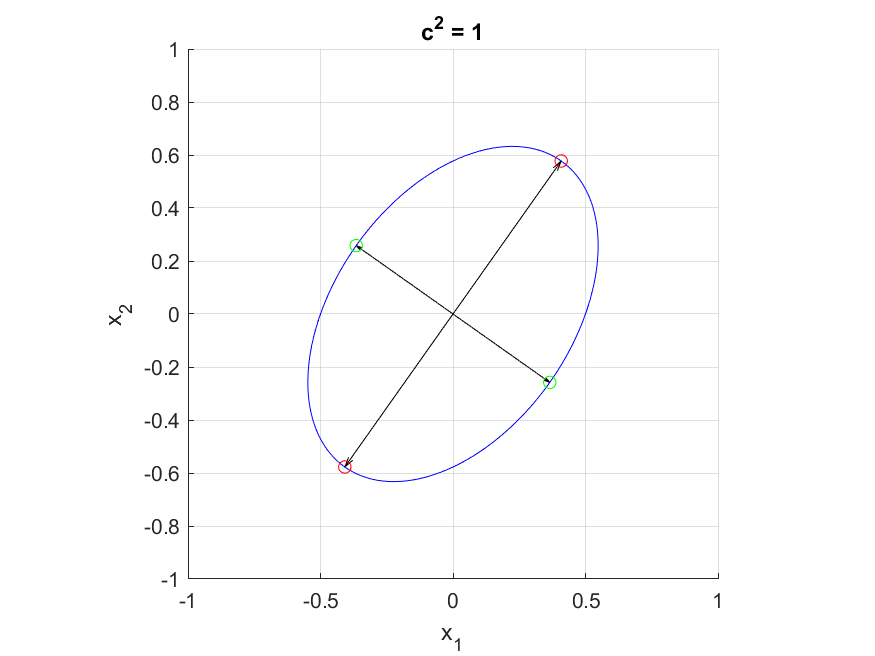
\includegraphics[scale=0.65]{./matlab/chapter-2/sol2.18.c1.png}
            \caption{When $c^2 = 1$}\label{fig:ellcis1}
        \end{figure}

        \begin{figure}[H]
            \centering
            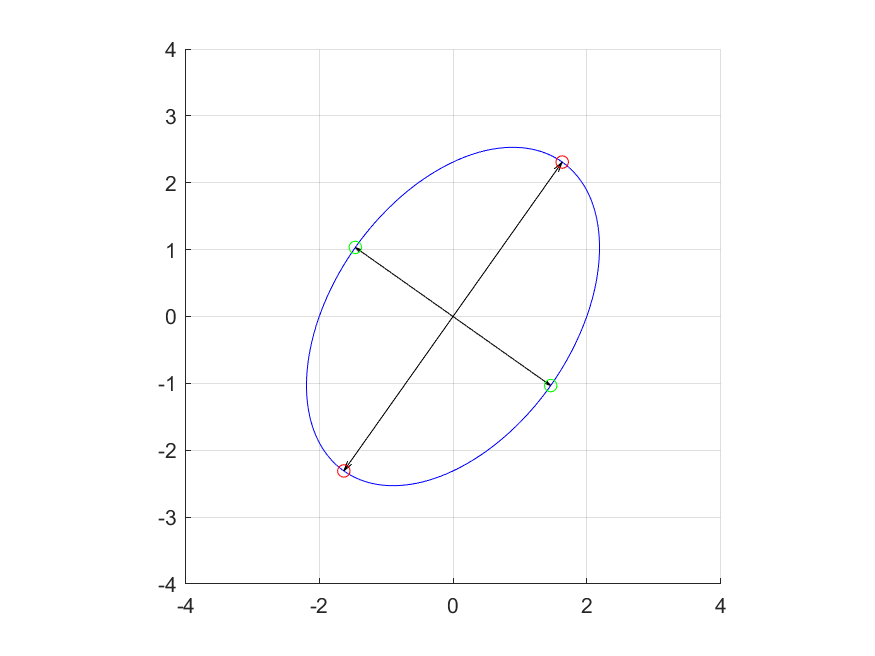
\includegraphics[scale=0.65]{./matlab/chapter-2/sol2.18.c4.png}
            \caption{When $c^2 = 4$}\label{fig:ellcis4}
        \end{figure}

        MATLAB code:
        \begin{lstlisting}
            A = [4 -sqrt(2); -sqrt(2) 3];
            [V,D] = eig(A);
            rref(A - D(1,1)*eye(width(A)))
            rref(A - D(2,2)*eye(width(A)))
            MyPlotEllipse(V,D,1,'sol2.18.c1')
            MyPlotEllipse(V,D,4,'sol2.18.c4')
        \end{lstlisting}

        \begin{lstlisting}
            function [] = MyPlotEllipse(V, D, c, fName)
    % Compute points corresponding to axis-oriented ellipse.
    % Where to center the ellipse.
    xc = 0;
    yc = 0;
    % The length in the major and minor axis.
    b = c/sqrt(D(1,1));
    a = c/sqrt(D(2,2));
    theta = acos(-V(:,1)'*[1 ; 0]); % acos(1/sqrt(3));
    
    t = linspace(0, 2*pi, 200);
    xt = b * cos(t) + xc;
    yt = a * sin(t) + yc;
    
    % Apply rotation by angle theta (in radians).
    cot = cos(theta); sit = sin(theta);
    x = xt * cot - yt * sit;
    y = xt * sit + yt * cot;

    hold on
        % Plot the ellipse.
        p=plot(x, y, '-', 'Color', 'blue');
        
        % Plot the vector for the major axis.
        quiver(0, 0, V(1,1), V(2,1), c, 'color', 'k');
        quiver(0, 0, -V(1,1), -V(2,1), c, 'color', 'k');
        
        % Plot the vector for the minor axis.
        quiver(0, 0, V(1,2), V(2,2), c, 'color', 'k');
        quiver(0, 0, -V(1,2), -V(2,2), c, 'color', 'k');
        
        % Plot red point for major axis.
        plot((c/sqrt(D(1,1)))*V(1,1), (c/sqrt(D(1,1)))*V(2,1), 'o', 'Color', 'red');
        plot(-(c/sqrt(D(1,1)))*V(1,1), -(c/sqrt(D(1,1)))*V(2,1), 'o', 'Color', 'red');
        
        % Plot green point for minor axis.
        plot((c/sqrt(D(2,2)))*V(1,2), (c/sqrt(D(2,2)))*V(2,2), 'o', 'Color', 'green');
        plot(-(c/sqrt(D(2,2)))*V(1,2), -(c/sqrt(D(2,2)))*V(2,2), 'o', 'Color', 'green');
        title(append('c^2 = ', num2str(c)))
        grid on
        pbaspect([1 1 1])
    hold off
    saved_file = append('.\applied-multivariate-statistics\solutions\chapter-2\', fName, '.png');
    saveas(p, saved_file, 'png')
end
        \end{lstlisting}